\chapter{Návrh}
Táto kapitola sa venuje návrhu architektúry budúcej aplikácie, s priblížením dvoch hlavných architektúr používaných pri tvorbe webových aplikácií. Následne sú porovnané a podľa výsledkov porovnania je vybraná taká, ktorá bude použitá pri vývoji aplikácie. V nasledujúcej sekcii sú vymedzené použité technológie budúcou aplikáciou. V neposlednom rade táto kapitola obsahuje návrh modelových tried a končí návrhom REST API, ktoré bude aplikácia používať pri komunikácii so serverom.

\section{Návrh architektúry}
Dôležitý aspekt pri návrhu aplikácie spočíva vo výbere architektúry, na ktorej bude aplikácia postavená. Na základe jej výberu sa odvíjajú technológie, ktorými bude daná aplikácia disponovať.

V nasledujúcich sekciách sú zdokumentované dva typy architektúr, z ktorých bude na základe porovnania a vlastných skúseností s tvorbou webových aplikácií vybraná jedna, ktorá bude definovať podobu budúcej webovej aplikácie.

\subsection{Architektúra MPA aplikácie}
MPA je skratka pre viac-stránkovú webovú aplikáciu. Takáto aplikácia vždy načíta celú stránku a zobrazí novú v prípade  interakcie s aplikáciou -- zvyčajne po odoslaní formuláru používateľom \cite{spa-vs-mpa-1}.

\subsubsection*{Priebeh komunikácie medzi serverom a klientom}
Celkový priebeh komunikácie medzi klientom a serverom zachytáva nasledujúci diagram s jeho popisom.

\begin{figure}[H]
	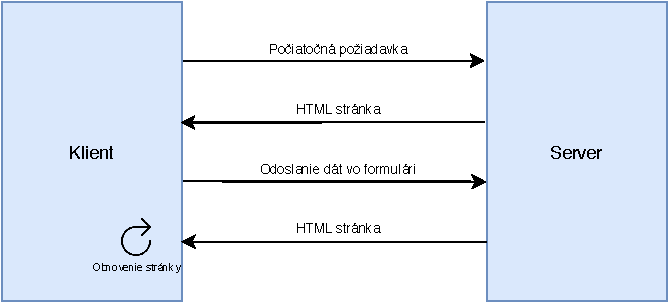
\includegraphics[width=1.0\textwidth]{media/navrh/MPA.pdf}
	\caption{Diagram znázorňujúci architektúru MPA aplikácií}\label{mpa-graf}
\end{figure}

\begin{enumerate}
	\item Klient požiada server o stránku
	\item Server vráti klientovi požadovanú stránku
	\item Klient vrátenú stránku serverom vykreslí
	\item Klient vyplní formulár, ktorý sa následne odošle na server
	\item Server prijme údaje od klienta, ktoré následne spracuje
	\item Po spracovaní údajov klientovi vráti späť stránku s aktualizovanými údajmi
	\item Klient túto stránku načíta, čím príde k obnoveniu stránky
\end{enumerate}

Technológia AJAX čiastočne rieši problém znovunačítavania celej stránky dynamickým aktualizovaním tých častí aplikácie, ktoré boli používateľom zmenené. Avšak zakomponovanie tejto technológie do MPA sťažuje a komplikuje celý vývojový proces aplikácie \cite{mpa-architektura}.

\subsubsection*{Výhody použitia MPA architektúry}

\begin{itemize}
	\item Jednoduchá optimalizácia stránok pre webové vyhľadávače \cite{spa-vs-mpa-1}
	\item Umožňuje jednoduchú správu informácií na jednotlivých stránkach \cite{spa-vs-mpa-3}
	\item Je potrebný menší rozsah nástrojov a znalostí narozdiel od vývoja SPA aplikácie \cite{spa-vs-mpa-2}
	\item Veľa dostupných riešení pre vývoj MPA aplikácií \cite{spa-vs-mpa-2}
\end{itemize}


\subsubsection*{Nevýhody použitia MPA architektúry}

\begin{itemize}
	\item Zvýšený čas načítavania stránok kvôli neustálemu obnovovaniu stránok (neplatí pri použití technológie AJAX) \cite{spa-vs-mpa-1}
	\item Znížený výkon aplikácie, kvôli neustálemu načítavaniu väčšieho množstva informácií naraz pred následným poslaním stránky používatelovi \cite{spa-vs-mpa-1}
	\item Úzka previazanosť vývoja aplikácie na strane servera a klienta, čo znemožňuje prípadné neskoršie nasadenie rôznych technológií \cite{spa-vs-mpa-2}
\end{itemize}


\subsection{Architektúra SPA aplikácie}
SPA je skratka pre single-page aplikáciu. Single-page aplikácia je aplikácia, ktorá nepotrebuje znovunačítanie stránky počas jej používania. Na tomto type architektúry sú postavené aplikácie ako Gmail\footnote{https://gmail.com}, Google Mapy\footnote{https://maps.google.com}, Facebook\footnote{https://facebook.com} či GitHub\footnote{https://github.com}. V tomto prípade sa o aktualizáciu obsahu na stránke nestará server, ale klient, zväčša pomocou frameworku\footnote{Sada podporných programov uľahčujúci vývoj aplikácie} bežiacom v prostredí webového prehliadača \cite{spa-vs-mpa-3}.

\subsubsection*{Priebeh komunikácie medzi serverom a klientom}
Celkový priebeh komunikácie medzi klientom a serverom zachytáva nasledujúci diagram s jeho popisom.

\begin{figure}[H]
	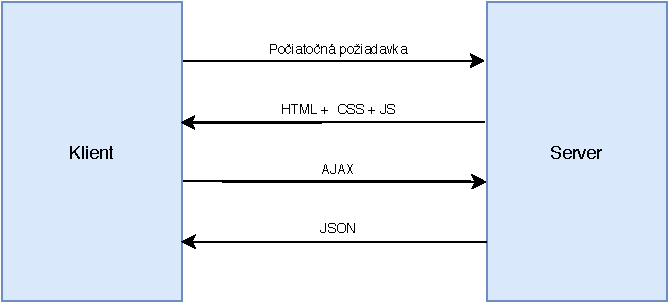
\includegraphics[width=1.0\textwidth]{media/navrh/SPA.pdf}
	\caption{Diagram znázorňujúci architektúru SPA aplikácií}\label{spa-graf}
\end{figure}

\begin{enumerate}
	\item Klient požiada server o stránku
	\item Server vráti klientovi požadovanú HTML stránku so všetkým obsahom aplikácie
	\item Klient vrátenú stránku serverom vykreslí
	\item Klient vyplní formulár, ktorý sa následne odošle na server pomocou AJAXu
	\item Server prijme údaje od klienta, ktoré následne spracuje
	\item Po spracovaní údajov server vráti späť klientovi aktualizované údaje (v JSON\footnote{Formát na výmenu dát medzi klientom a serverom \cite{co-je-json} } formáte)
	\item Klient zahodí staré údaje na stránke a nahradí ich novými, čím príde k obnoveniu údajov ale nie stránky
\end{enumerate}


\subsubsection*{Výhody použitia SPA architektúry}

\begin{itemize}
	\item Rýchlosť a responzívnosť aplikácie založenej na aktualizovaní iba tej časti aplikácie, ktorá sa zmenila \cite{spa-vs-mpa-1}
	\item Minimálna previazanosť kódu aplikácie na strane servera a klienta, čo umožňuje jednoduchú správu používaných knižníc bez ovplyvnenia ďalších častí aplikácie \cite{spa-vs-mpa-2}
	\item Zjednodušení proces vývoja, nakoľko sa o vykreslenie obsahu nestará server ale klientský framework \cite{spa-vs-mpa-3}
\end{itemize}


\subsubsection*{Nevýhody použitia SPA architektúry}

\begin{itemize}
	\item Ťažká optimalizácia aplikácie pre webové vyhľadávače, nakoľko o vykreslenie obsahu sa stará Javascript\footnote{Programovací jazyk bežiaci vo webovom prehliadači}, ktorý webové vyhľadávače neinterpretujú \cite{spa-vs-mpa-1}
	\item Prvné načítanie aplikácie trvá dlhší čas v porovnaní s MPA architektúrou, pretože pri prvom navštívení aplikácie sa musí všetok obsah aplikácie stiahnuť do zariadenia
	\item Nemožnosť zobrazenia aplikácie pri vypnutom Javascripte vo webovom prehliadači \cite{spa-vs-mpa-2}
	\item Pri komplexnejšej aplikácii bude aplikácia zaberať viac pamäte zariadenia, z ktorého je zobrazovaná, nakoľko všetok obsah aplikácie je stiahnutý v zariadení \cite{spa-vs-mpa-3}
\end{itemize}



\subsection{Porovnanie a voľba architektúry}





\section{Návrh technológií}


\subsection{Back-end technológie}


\subsection{Front-end technológie}




\section{Návrh modelových tried}




\section{Návrh REST API}